%-------------------------------------------
\begin{frame}{\raisebox{-1ex}{\includegraphics[height=0.8cm]{shared/logo-github.png}} }
%-------------------------------------------
\begin{columns}
\begin{column}{0.5\textwidth}
\begin{exampleblock}{2: create branch1}
    \begin{center}
    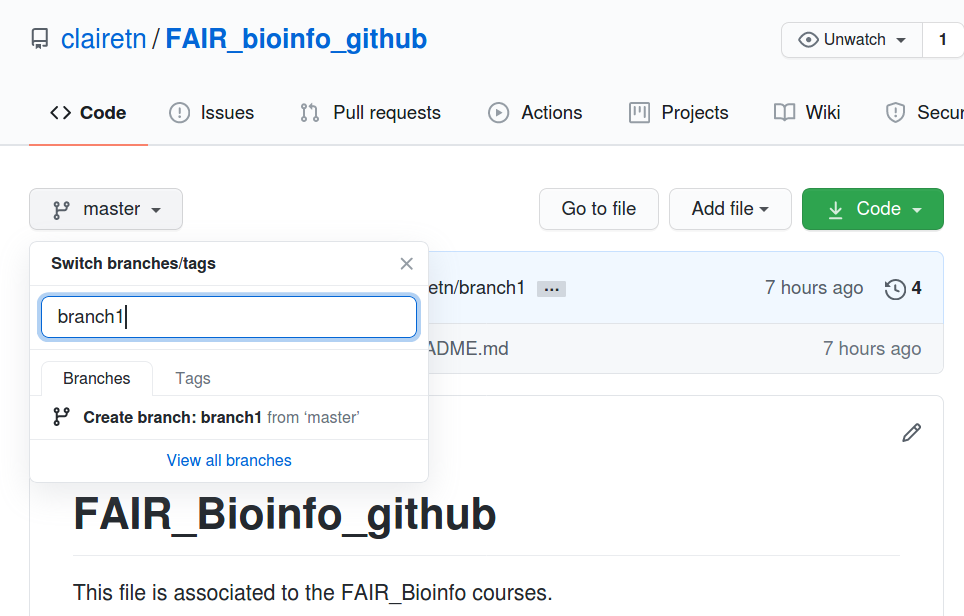
\includegraphics[height=3.8cm]{05_history/Images/FAIR_github_branch1.png}
    \end{center}
\end{exampleblock}
\end{column}
\begin{column}{0.46\textwidth}
\begin{exampleblock}{branch1 created}
    \begin{center}
    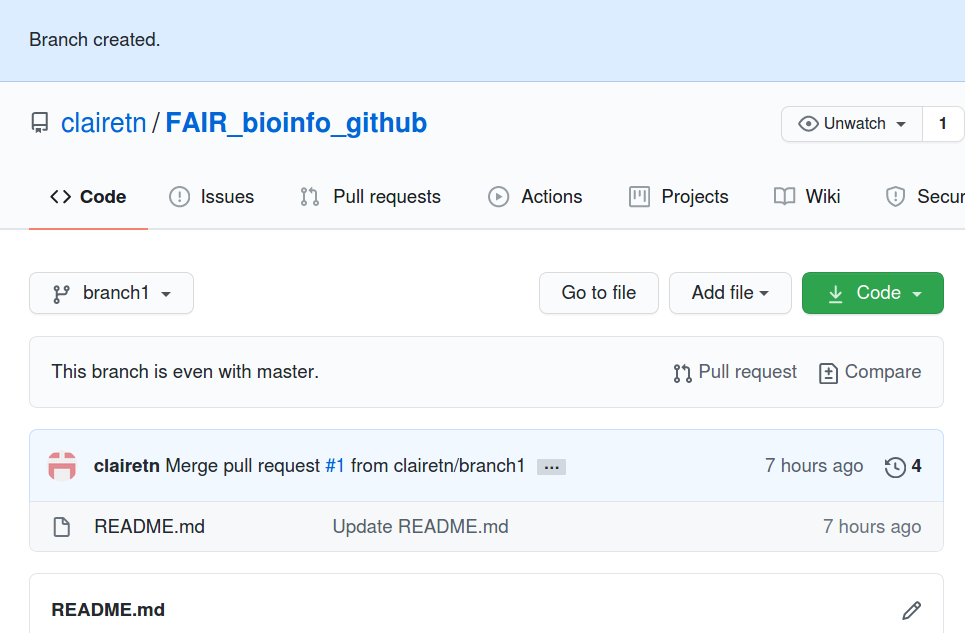
\includegraphics[height=3.6cm]{05_history/Images/FAIR_github_branch1ok.png}
    \end{center}
\end{exampleblock}
\end{column}
\end{columns}
\end{frame}
%-------------------------------------------
\begin{frame}{\raisebox{-1ex}{\includegraphics[height=0.8cm]{shared/logo-github.png}} }
%-------------------------------------------
\begin{columns}
\begin{column}{0.48\textwidth}
\begin{exampleblock}{3: make change (Edit, click pen)}
    \begin{center}
    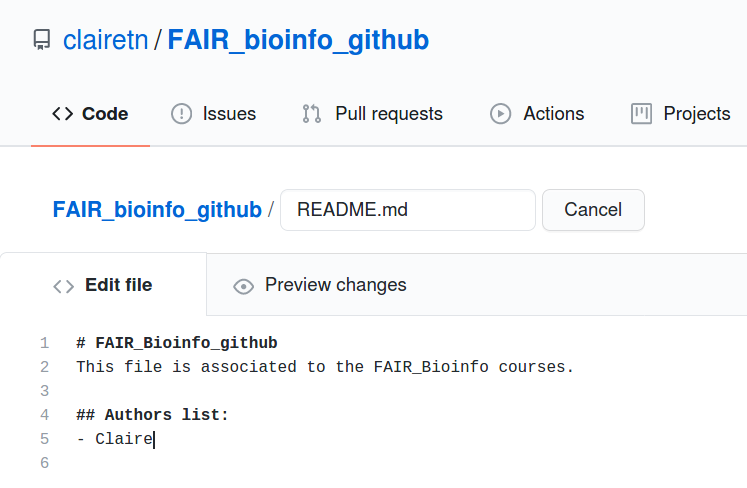
\includegraphics[height=3.6cm]{05_history/Images/FAIR_github_EditFile.png}
    \end{center}
\end{exampleblock}
\end{column}
\begin{column}{0.48\textwidth}
\begin{exampleblock}{4: commit (bottom page)}
    \begin{center}
    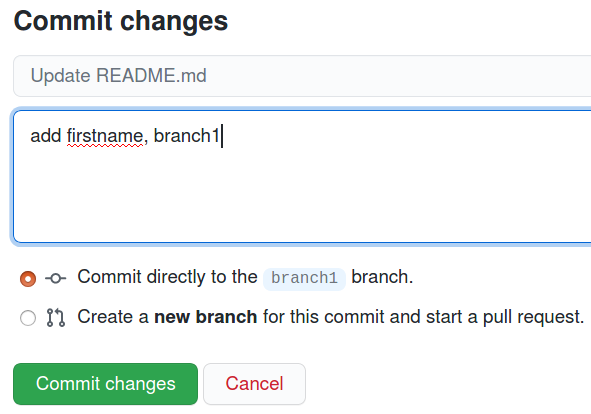
\includegraphics[height=3.6cm]{05_history/Images/FAIR_github_Commit.png}
    \end{center}
\end{exampleblock}
% TODO ajouter une flèche orange vers le bas pour indiquer que la dias suivante en en bas de la page 
\end{column}
\end{columns}
\end{frame}
%-------------------------------------------
\begin{frame}{\raisebox{-1ex}{\includegraphics[height=0.8cm]{shared/logo-github.png}} }
%-------------------------------------------
\begin{columns}
\begin{column}{0.48\textwidth}
\begin{exampleblock}{5: Compare}
    \begin{center}
    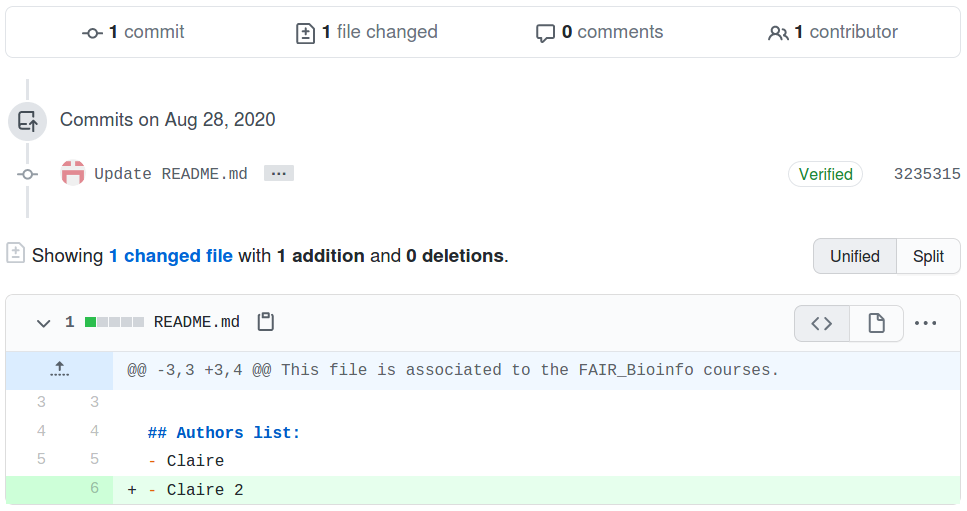
\includegraphics[height=3cm]{05_history/Images/FAIR_github_compareBranch1.png}
    \end{center}
\end{exampleblock}
 take some time to appear ...
\end{column}
\begin{column}{0.48\textwidth}
\begin{exampleblock}{6: Pull request commit}
    \begin{center}
    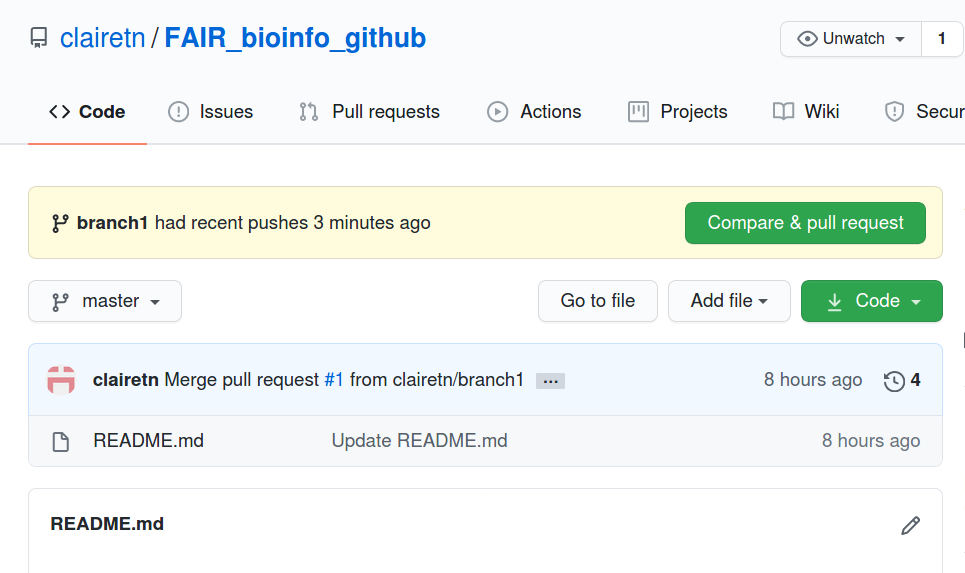
\includegraphics[height=2.8cm]{05_history/Images/FAIR_github_comparePull.png}
    \end{center}
\end{exampleblock}
\end{column}
\end{columns}
\end{frame}
%-------------------------------------------
\begin{frame}{\raisebox{-1ex}{\includegraphics[height=0.8cm]{shared/logo-github.png}} }
%-------------------------------------------
\begin{columns}
\begin{column}{0.48\textwidth}
\begin{exampleblock}{7: Merge branch1}
    \begin{center}
    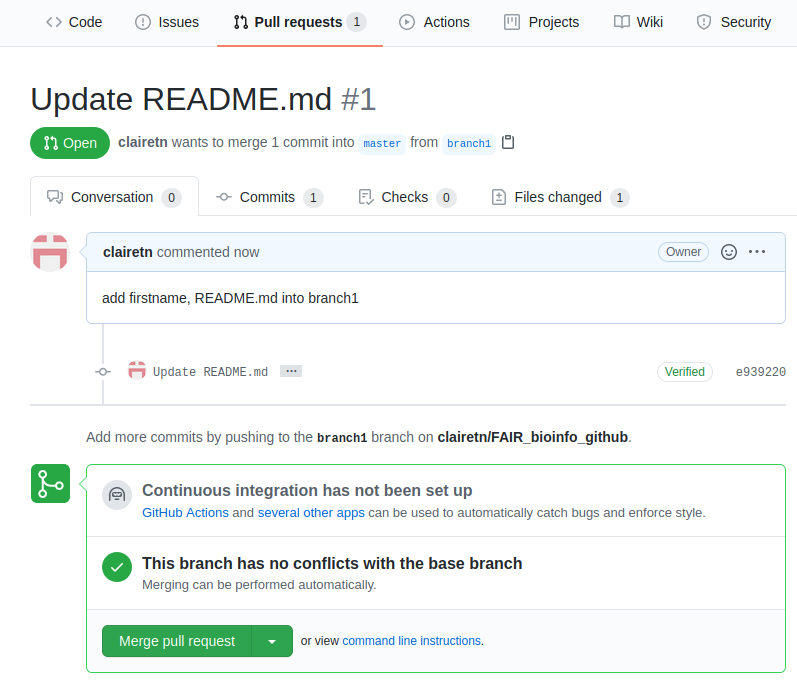
\includegraphics[height=4.5cm]{05_history/Images/FAIR_github_PullRequestBranch1.png}
    \end{center}
\end{exampleblock}
\end{column}
\begin{column}{0.48\textwidth}
\begin{exampleblock}{8: Pull request merge}
    \begin{center}
    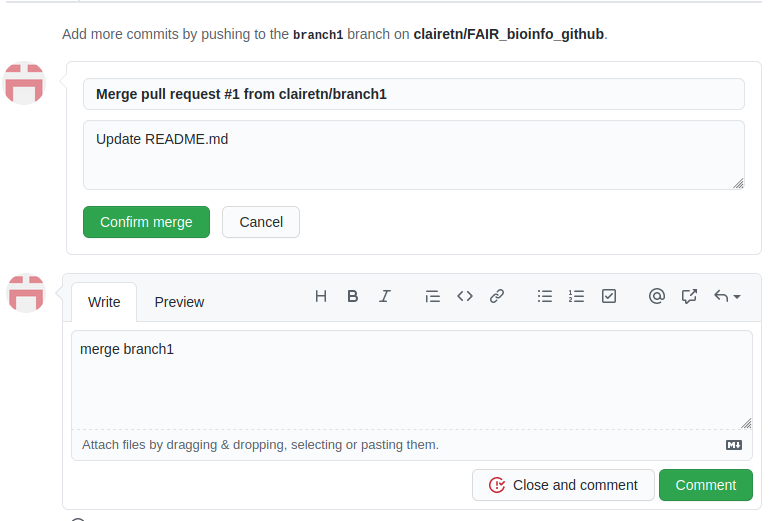
\includegraphics[height=3.5cm]{05_history/Images/FAIR_github_MergeBranch1.png}
    \end{center}
\end{exampleblock}
\end{column}
\end{columns}
\end{frame}
%-------------------------------------------
\begin{frame}{\raisebox{-1ex}{\includegraphics[height=0.8cm]{shared/logo-github.png}} }
%-------------------------------------------
\begin{columns}
\begin{column}{0.49\textwidth}
\begin{exampleblock}{Merge success}
    \begin{center}
    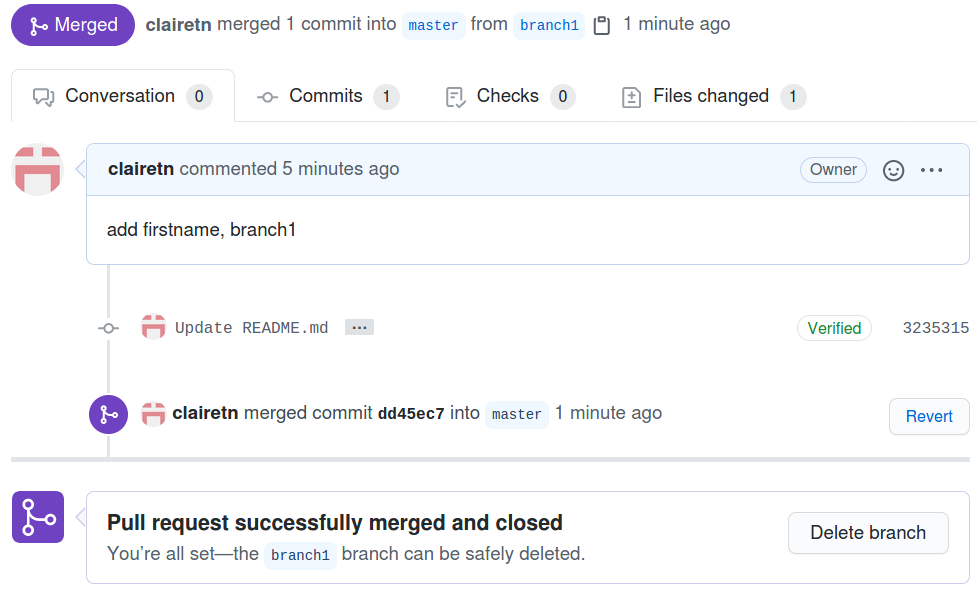
\includegraphics[height=3.5cm]{05_history/Images/FAIR_github_MergeSucceed.png}
    \end{center}
\end{exampleblock}
\end{column}
\begin{column}{0.49\textwidth}
\begin{exampleblock}{9: Delete branch1}
    \begin{center}
    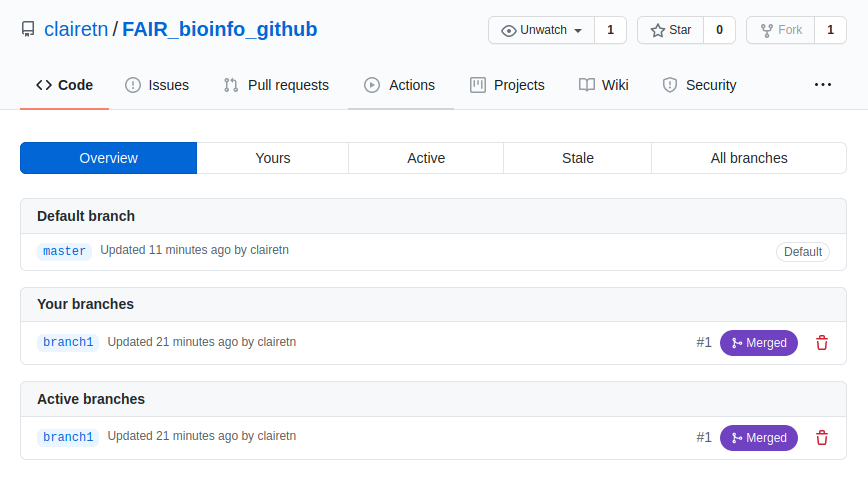
\includegraphics[height=3.4cm]{05_history/Images/FAIR_github_DeleteBranch1.png}
    \end{center}
\end{exampleblock}
\end{column}
\end{columns}
\end{frame}